\documentclass{cmn}

\newlength\width
\setlength\width{12mm}
\newlength\height
\setlength\height{9mm}
\newlength\ySep
\setlength\ySep{24mm}

\newcommand\drawArray{
  \draw (0,0) -- ++(7*\width,0) -- ++(0,\height) -- ++(-7*\width,0) -- cycle;
  \foreach \i in {1,2,3,5,6} {
    \draw (\i*\width,0) -- ++(0,\height);
  }
  \foreach \i/\label in {0/$n$,1/$n-1$,2/$n-2$,3.5/$\dots$,5/$2$,6/$1$} {
    \node at (\width/2+\i*\width,\height/2) {\small\label};
  }
}

\begin{document}
  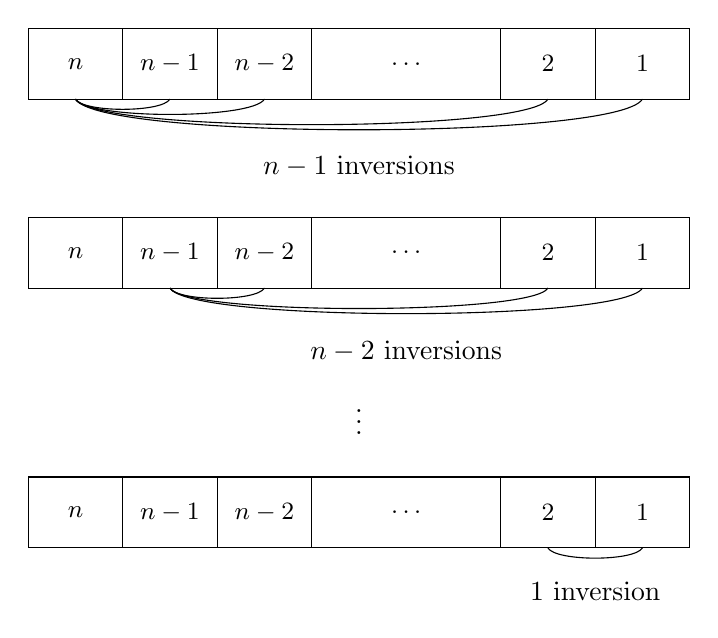
\begin{tikzpicture}
    \begin{scope}
      \drawArray

      \foreach \n/\control in {1/2mm,2/3mm,5/5mm,6/6mm} {
        \draw (\width/2,0) .. controls +(-60:\control) and +(-120:\control) .. ++(\n*\width,0);
      }

      \node at (3.5*\width,-8.5mm) {$n-1$ inversions};
    \end{scope}

    \begin{scope}[yshift=-\ySep]
      \drawArray

      \foreach \n/\control in {1/2mm,4/4mm,5/5mm} {
        \draw (3*\width/2,0) .. controls +(-60:\control) and +(-120:\control) .. ++(\n*\width,0);
      }

      \node at (4*\width,-8mm) {$n-2$ inversions};

      \node at (3.5*\width,-16mm) {$\vdots$};
    \end{scope}

    \begin{scope}[yshift=-2.375*\ySep]
      \drawArray

      \foreach \n/\control in {1/2mm} {
        \draw (11*\width/2,0) .. controls +(-60:\control) and +(-120:\control) .. ++(\n*\width,0);
      }

      \node at (6*\width,-5.5mm) {$1$ inversion};
    \end{scope}
  \end{tikzpicture}
\end{document}
